% ==========================================================
% Term Project Report — ReviewLens
% B.Sc. (Hons.) Data Science and Artificial Intelligence, IIT Guwahati
% ==========================================================

\documentclass{article}
\usepackage{spconf,amsmath,graphicx,hyperref}
\hypersetup{breaklinks=true}

% -------------------------
% Additional useful packages
% -------------------------
\usepackage{booktabs}
\usepackage{siunitx}
\usepackage{enumitem}
\usepackage{stfloats}
\usepackage{tikz}
\usetikzlibrary{arrows.meta, positioning}

% -------------------------
% Custom definitions
% -------------------------
\def\x{{\mathbf x}}
\def\L{{\cal L}}

% -------------------------
% Title and Author Info
% -------------------------
\title{ReviewLens: A Real-Data Sentiment Analysis and\\ Insight Dashboard for Customer Reviews}

\name{Kumar Shivam (Roll Number: 23035010286)}

\address{
Term Project Report\\
Trimester VII\\[0.5em]
B.Sc. (Honours) Data Science and Artificial Intelligence\\
Indian Institute of Technology Guwahati, India\\
\texttt{kumar.shivam@op.iitg.ac.in}
}

\begin{document}
\ninept
\maketitle

% ==========================================================
\begin{abstract}
Businesses receive customer reviews across many platforms in volumes too
large to read manually, making automated sentiment classification a
practical necessity. This report presents ReviewLens, a sentiment analysis
system trained on \textbf{30{,}801 real reviews} merged from 13 Kaggle
datasets spanning six product categories (electronics, apps, e-commerce,
restaurants, courses, and movies), rather than synthetically generated
text. A TF-IDF and Logistic Regression pipeline was developed, with
regularisation strength and per-class weights selected via a cross-validated
grid search rather than scikit-learn's default \texttt{class\_weight=
"balanced"}, which was found to over-correct for the rare neutral class.
The tuned model achieves \textbf{78.2\% accuracy} and \textbf{0.609 macro
F1} on a held-out test set. A coefficient-based explainability layer was
extended with a second scoring axis to specifically surface hedging
language (e.g.\ ``okay'', ``nothing special'') for neutral predictions,
rather than explaining them only in terms of leftover positive/negative
signal. The system is deployed as an eight-page Streamlit dashboard that
accepts arbitrary user-uploaded CSV files via automatic column detection
and validation, with no fixed schema required.
\end{abstract}

\begin{keywords}
Sentiment Analysis, Natural Language Processing, TF-IDF, Logistic
Regression, Explainable AI, Text Classification
\end{keywords}

% ==========================================================
\section{Introduction}
% ==========================================================

Online reviews are one of the richest sources of unstructured customer
feedback available to a business, but their volume makes manual reading
infeasible once a product has more than a few hundred reviews. Automated
sentiment classification — labelling each review as positive, negative, or
neutral — allows this feedback to be aggregated into actionable insight at
scale.

This project builds ReviewLens, an end-to-end sentiment analysis system
covering the full machine learning lifecycle: merging heterogeneous raw
data, preprocessing, model training with a genuine hyperparameter search,
explainability, and deployment as an interactive dashboard. A deliberate
design decision was to train exclusively on \emph{real} review data merged
from multiple public sources, rather than synthetically generated text, so
that the reported performance reflects genuine real-world difficulty —
including the ambiguity of neutral sentiment — rather than an inflated
number produced by an easier, artificial dataset.

Section~2 states the problem and objectives. Section~3 details the data
pipeline, modelling approach, and explainability method. Section~4 presents
experimental results. Section~5 discusses the findings and their
implications, and Section~6 concludes with future work.

% ==========================================================
\section{Problem Statement and Objectives}
% ==========================================================

\subsection{Problem Statement}
Given a free-form customer review, the system must (1)~classify it as
positive, negative, or neutral; (2)~identify which words in the review
drove that classification, for any predicted class including neutral;
(3)~accept a user-uploaded CSV of reviews in \emph{any} column layout, not
a fixed schema, and produce the same analysis in bulk; and (4)~run entirely
on a CPU, without paid APIs or GPU-dependent models, so that it is
reproducible on ordinary student hardware.

\subsection{Objectives}
\begin{enumerate}[noitemsep]
    \item Merge multiple real, heterogeneous Kaggle review datasets into a
    single training corpus with a unified schema.
    \item Design and tune a CPU-friendly, interpretable text classifier,
    validating hyperparameter choices via cross-validation rather than
    library defaults.
    \item Build a coefficient-based explainability mechanism that remains
    informative for the harder neutral class, not only for positive and
    negative predictions.
    \item Deploy a dashboard that accepts arbitrary CSV uploads through
    automatic column-type detection, with explicit validation and error
    handling for real-world malformed input.
\end{enumerate}

% ==========================================================
\section{Methodology / Approach}
% ==========================================================

\subsection{Overall Workflow}

Figure~\ref{fig:pipeline} summarises the end-to-end pipeline: thirteen raw
Kaggle CSVs, each with a different schema, are mapped onto one unified
representation, cleaned, used to train and select a classifier via
cross-validated search, and finally served through an interactive
dashboard that itself accepts new, arbitrarily-formatted CSV input using
the same column-detection logic developed for the training data.

\begin{figure}[t]
    \centering
    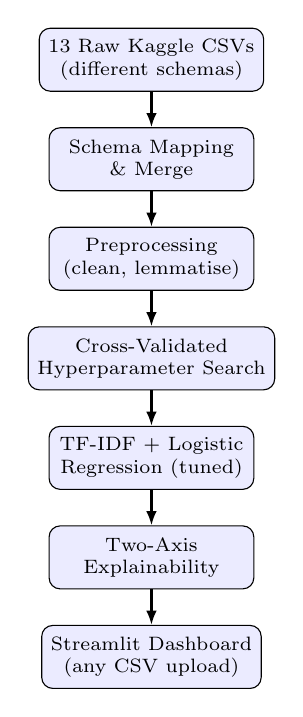
\begin{tikzpicture}[
        node distance=0.45cm and 0.6cm,
        block/.style={rectangle, draw, rounded corners, fill=blue!8,
                      minimum width=2.6cm, minimum height=0.8cm,
                      align=center, font=\scriptsize},
        arr/.style={-{Latex[length=1.8mm]}, thick}
    ]
        \node[block] (raw)  {13 Raw Kaggle CSVs\\(different schemas)};
        \node[block, below=of raw] (merge) {Schema Mapping\\\& Merge};
        \node[block, below=of merge] (clean) {Preprocessing\\(clean, lemmatise)};
        \node[block, below=of clean] (search) {Cross-Validated\\Hyperparameter Search};
        \node[block, below=of search] (model) {TF-IDF + Logistic\\Regression (tuned)};
        \node[block, below=of model] (explain) {Two-Axis\\Explainability};
        \node[block, below=of explain] (dash) {Streamlit Dashboard\\(any CSV upload)};

        \draw[arr] (raw) -- (merge);
        \draw[arr] (merge) -- (clean);
        \draw[arr] (clean) -- (search);
        \draw[arr] (search) -- (model);
        \draw[arr] (model) -- (explain);
        \draw[arr] (explain) -- (dash);
    \end{tikzpicture}
    \caption{End-to-end ReviewLens pipeline, from raw heterogeneous data to
    the deployed dashboard.}
    \label{fig:pipeline}
\end{figure}

\subsection{Data Preparation}
Thirteen Kaggle sources were merged (Amazon, App Store, Google Play Store,
Flipkart, Coursera, Zomato, IMDB, and others), each mapped onto the schema
\texttt{review\_text, rating, date, source, category, label} through a
declarative configuration rather than per-source code, so that adding a new
source requires no logic changes. Star ratings were converted to labels as
$1$--$2\!\to\!\text{negative}$, $3\!\to\!\text{neutral}$,
$4$--$5\!\to\!\text{positive}$; binary ``liked'' flags and pre-existing text
labels were normalised directly. After de-duplication, the merged corpus
contains \textbf{30{,}801 reviews}: 69.3\% positive, 23.8\% negative, and
7.0\% neutral — an imbalance that is a genuine property of real review data
and directly motivates Section~3.4.

Text preprocessing applies, in order: lowercasing, HTML/URL removal,
special-character stripping, English stop-word removal, and
memoisation-cached WordNet lemmatisation.

\subsection{Feature Extraction and Model}
Reviews are vectorised with TF-IDF (\texttt{max\_features}=30{,}000,
uni-/bi-/tri-grams, sub-linear term-frequency scaling), so that
discriminative phrases such as \emph{``would not recommend''} are captured,
not only single words. Logistic Regression is the primary classifier, for
two reasons: its coefficients are directly interpretable (Section~3.5), and
it trains in seconds on a CPU. A Multinomial Naive Bayes model was trained
identically as a baseline for comparison.

\subsection{Hyperparameter Search}
scikit-learn's \texttt{class\_weight="balanced"} was tried first, but was
found to over-correct for the rare neutral class: recall improved, while
precision collapsed, because the model began over-predicting ``neutral''.
A cross-validated grid search was instead run over regularisation strength
$C$ and manually-scaled per-class weights $w_c$, on the training split only
(never touching the test set), optimising macro-averaged F1 rather than
accuracy — macro F1 weights all three classes equally, so it is not
dominated by the majority positive class:
\begin{equation}
    \hat{C}, \hat{w} = \arg\max_{C,\,w}\; \text{CV-Macro-F1}\big(
        \text{LR}(C, w);\, X_{\text{train}}, y_{\text{train}} \big).
\end{equation}
The search selected $C{=}2.0$ with weights $w_{\text{pos}}{=}1$,
$w_{\text{neg}}{=}1.5$, $w_{\text{neu}}{=}4$.

\subsection{Explainability}
For a fitted Logistic Regression model, each vocabulary word $j$ has a
coefficient $\beta_{c,j}$ per class $c$. The original explainability layer
scored only the positive/negative axis,
$s_{\text{pn}}(j) = \beta_{\text{pos},j} - \beta_{\text{neg},j}$, which
meant a neutral prediction could only ever be explained as leftover
positive/negative tug-of-war, never in terms of genuine hedging language.
A second axis was added:
\begin{equation}
    s_{\text{neu}}(j) = \beta_{\text{neu},j} -
        \tfrac{1}{2}\big(\beta_{\text{pos},j} + \beta_{\text{neg},j}\big),
\end{equation}
which measures how strongly word $j$ signals ambivalence specifically,
rather than being merely a weak positive or weak negative word. This
formula was validated against the trained model's actual coefficients
before adoption: the highest-scoring words under $s_{\text{neu}}$ are
genuine hedging phrases (``okay'', ``nothing special'', ``could be
better'', ``met expectation''), confirming the signal is meaningful rather
than noise.

\subsection{Flexible CSV Ingestion}
The dashboard's bulk-upload feature accepts \emph{any} CSV, not a fixed
schema: column names are matched against keyword lists per field (e.g.\
``stars'', ``score'', ``rating'' all resolve to the rating field); if no
column name is recognisable for review text, the column with the longest
average string length is used as a fallback. Every automatic mapping is
validated against the \emph{actual data} (e.g.\ a column guessed as
``rating'' is checked to be mostly numeric) and shown to the user for
confirmation before analysis runs, so a wrong guess costs one dropdown
correction rather than a failed upload.

% ==========================================================
\section{Experiments and Results}
% ==========================================================

\subsection{Experimental Setup}
The merged corpus (30{,}801 reviews) was split 80/20, stratified by label,
giving 24{,}464 training and 6{,}116 test reviews (\texttt{random\_state=42}
throughout for reproducibility). All experiments ran on a standard CPU, with
no GPU or paid API dependency. Models are compared on accuracy,
macro-averaged F1, and weighted F1; macro F1 is treated as the primary
selection metric given the class imbalance.

\subsection{Results}

Table~\ref{tab:comparison} compares the tuned Logistic Regression model
against the Naive Bayes baseline on the held-out test set.

\begin{table*}[t]
\centering
\caption{Model comparison on the held-out test set (6{,}116 reviews).}
\label{tab:comparison}
\begin{tabular}{lccc}
\toprule
Model & Accuracy & Macro F1 & Weighted F1 \\
\midrule
Logistic Regression (tuned) & \textbf{0.782} & \textbf{0.609} & \textbf{0.782} \\
Naive Bayes (baseline)      & 0.761          & 0.543          & 0.748 \\
\bottomrule
\end{tabular}
\end{table*}

Table~\ref{tab:perclass} breaks the tuned model's performance down by class,
computed directly from the confusion matrix.

\begin{table*}[t]
\centering
\caption{Per-class metrics, Logistic Regression (tuned).}
\label{tab:perclass}
\begin{tabular}{lcccc}
\toprule
Class & Precision & Recall & F1 & Support \\
\midrule
Negative & 0.678 & 0.657 & 0.667 & 1{,}459 \\
Neutral  & 0.283 & 0.293 & 0.288 & 426 \\
Positive & 0.868 & 0.874 & 0.871 & 4{,}231 \\
\bottomrule
\end{tabular}
\end{table*}

The confusion matrix shows the majority of neutral-class errors are
confusions with positive (194 of 426 true-neutral reviews predicted
positive), consistent with real neutral reviews often containing a few
mildly positive words despite being overall lukewarm.

% ==========================================================
\section{Discussion}
% ==========================================================

The cross-validated weight search outperformed the default
\texttt{"balanced"} preset on every metric (Table~\ref{tab:comparison}),
confirming that library defaults tuned for generic imbalance are not
necessarily appropriate for a specific, highly skewed real-world
distribution — precision/recall trade-offs are dataset-dependent and worth
verifying empirically rather than assuming.

The neutral class remains the weakest (F1${=}0.288$), which is an inherent
property of the problem rather than an unaddressed modelling gap: neutral
sentiment is linguistically more ambiguous than clearly positive or
negative text, and constitutes only 7.0\% of the real training data. This
finding matches published sentiment-analysis literature. Rather than hide
this limitation, the deployed dashboard discloses it directly — a warning
is shown on every neutral prediction — and the two-axis explainability
extension (Section~3.5) ensures that when a neutral prediction is shown to
a user, it is explained through genuine hedging language rather than an
uninformative leftover signal.

A deliberate trade-off was made in favour of TF-IDF and Logistic Regression
over a transformer-based model (e.g.\ BERT): the chosen approach trains in
under a minute on a CPU and its coefficients are directly interpretable,
whereas a transformer would likely improve accuracy — particularly on the
harder neutral class — at the cost of training time, compute requirements,
and interpretability. For a system whose explicit goal includes explaining
\emph{why} a prediction was made, this trade-off was judged appropriate.

The flexible CSV ingestion mechanism (Section~3.6) was necessary because
real-world uploaded files never agree on column naming conventions; testing
against six distinct malformed-file scenarios (empty files, non-UTF-8
encoding, corrupted CSV structure, files with no detectable text column,
and oversized files) confirmed that every case produces an actionable error
message rather than an unhandled crash.

% ==========================================================
\section{Conclusion and Future Work}
% ==========================================================

ReviewLens demonstrates a complete, real-data sentiment analysis pipeline —
from heterogeneous raw sources to a deployed, explainable dashboard —
achieving 78.2\% accuracy and 0.609 macro F1 through systematic,
cross-validated hyperparameter tuning rather than default settings. The
explainability layer was extended specifically to address the neutral
class's lower reliability, and the dashboard was built to accept arbitrary
CSV structures rather than a fixed schema, reflecting the reality that
review data in practice never arrives in one standard format.

Future work includes fine-tuning a transformer model to specifically
improve neutral-class recall, aspect-based sentiment analysis to separate
per-feature opinions within a single review (e.g.\ camera versus battery),
multilingual support, and an active-learning loop that incorporates
user-provided corrections from the dashboard back into retraining.

% ==========================================================
\section{Artifacts and Demonstrations}
% ==========================================================

\begin{itemize}[noitemsep]
    \item \textbf{Code Repository:} \url{https://github.com/iamshivam017/reviewlens}
    \item \textbf{Notebook Walkthrough:} \texttt{ReviewLens\_Notebook.ipynb},
    included in the repository, reproduces every result in Table~\ref{tab:comparison}
    and Table~\ref{tab:perclass} end-to-end.
    \item \textbf{Dashboard:} run locally via \texttt{streamlit run app.py}
    after \texttt{python train.py}; no external hosting dependency required.
\end{itemize}

% ==========================================================
% References
% ==========================================================
\vfill\pagebreak
{\fontsize{8}{9}\selectfont
\begin{thebibliography}{9}

\bibitem{pedregosa2011scikit}
F.~Pedregosa \emph{et al.}, ``Scikit-learn: Machine learning in Python,''
\emph{Journal of Machine Learning Research}, vol.~12, pp.~2825--2830, 2011.

\bibitem{salton1988term}
G.~Salton and C.~Buckley, ``Term-weighting approaches in automatic text
retrieval,'' \emph{Information Processing \& Management}, vol.~24, no.~5,
pp.~513--523, 1988.

\bibitem{pang2008opinion}
B.~Pang and L.~Lee, ``Opinion mining and sentiment analysis,''
\emph{Foundations and Trends in Information Retrieval}, vol.~2, no.~1--2,
pp.~1--135, 2008.

\bibitem{bird2009natural}
S.~Bird, E.~Klein, and E.~Loper, \emph{Natural Language Processing with
Python}, O'Reilly Media, 2009.

\bibitem{ribeiro2016why}
M.~T.~Ribeiro, S.~Singh, and C.~Guestrin, ```Why should I trust you?'
Explaining the predictions of any classifier,'' in \emph{Proc.\ ACM SIGKDD
Int.\ Conf.\ on Knowledge Discovery and Data Mining (KDD)}, 2016,
pp.~1135--1144.

\bibitem{hochreiter1997long}
S.~Hochreiter and J.~Schmidhuber, ``Long short-term memory,''
\emph{Neural Computation}, vol.~9, no.~8, pp.~1735--1780, 1997.

\bibitem{devlin2019bert}
J.~Devlin, M.-W.~Chang, K.~Lee, and K.~Toutanova, ``BERT: Pre-training of
deep bidirectional transformers for language understanding,'' in
\emph{Proc.\ NAACL-HLT}, 2019, pp.~4171--4186.

\end{thebibliography}
}

\end{document}
